\documentclass[11pt]{article}


%%%%%%%%%%%%%%%%%%%%%%%%%%%%%%%%
%%%%%%%%%%%%%%%%%%%%%%%%%%%%%%%%
%% PACKAGES %%%%%%%%%%%%%%%%%%%%
%%%%%%%%%%%%%%%%%%%%%%%%%%%%%%%%
%%%%%%%%%%%%%%%%%%%%%%%%%%%%%%%%

\usepackage[margin=0.9in, top=0.8in, bottom=1.0in]{geometry}
\usepackage[charter]{mathdesign} % Main font.
\usepackage{qpxmath} % Palatino-based math font, better than charter.
\usepackage[scaled]{beramono} % Lovely monospace font
\usepackage[T1]{fontenc}
\usepackage{amsmath}
\usepackage{mathtools}
\usepackage{mathdots}
\usepackage{graphicx}
\usepackage[update,prepend]{epstopdf} % To use eps files.
\usepackage{microtype}
\usepackage{titlesec} % Custom section headings.
\usepackage{xcolor}
\usepackage{xspace}
\usepackage{xfrac}
\usepackage{calc}
\usepackage{listings} % Code listings.
\usepackage{matlab-prettifier} % MATLAB code listings
\usepackage[labelfont=bf]{caption} % Figure captions.
\usepackage{enumitem} % Fine tuning enumerations.
\usepackage{floatrow} % Captions to the right of figures.
\usepackage[numbers]{natbib}
\usepackage{wrapfig}

% Packages to makes tables pretty.
\usepackage{array}
\usepackage{booktabs}
\setlength{\heavyrulewidth}{1.5pt}
\setlength{\abovetopsep}{4pt}

% Fancyhdr package stuff...
\usepackage{fancyhdr}
\setlength{\headheight}{0pt}
\setlength{\footskip}{50pt}
\renewcommand{\headrulewidth}{0pt}
\renewcommand{\footrulewidth}{0pt}

%%%%%%%%%%%%%%%%%%%%%%%%%%%%%%%%
%%%%%%%%%%%%%%%%%%%%%%%%%%%%%%%%
%% SETTINGS %%%%%%%%%%%%%%%%%%%%
%%%%%%%%%%%%%%%%%%%%%%%%%%%%%%%%
%%%%%%%%%%%%%%%%%%%%%%%%%%%%%%%%

% Path to look for graphics
\graphicspath{{../images/}}
%\epstopdfsetup{outdir=../images/}

% Caption spacing
\setlength{\abovecaptionskip}{0pt}

% List spacing
\setlist{noitemsep}

% Math operator font
\DeclareSymbolFont{sfoperators}{OT1}{cmss}{m}{n}
\DeclareSymbolFontAlphabet{\mathsf}{sfoperators}
\makeatletter
\def\operator@font{\mathgroup\symsfoperators}
\makeatother

%% No indent all paragraphs
%\setlength{\parindent}{0in}

% Figure references
\newcommand{\figref}[1]{Figure~\ref{#1}}

% Special format section headings
\titleformat{\section}%
	{\large\bf\scshape}% Text formatting
	{\arabic{section}}% Number
	{1em}% Space between number and text
	{}% Code before
	[]% Code after
\titleformat{\subsection}%
	{\normalsize\bf\scshape}% Text formatting
	{\arabic{section}.\arabic{subsection}}% Number
	{1em}% Space between number and text
	{}% Code before
	[]% Code after
%\titleformat{\subsubsection}%
%	{\color{blue}}% Text formatting
%	{\arabic{subsubsection} $\rightarrow$}% Number
%	{1em}% Space between number and text
%	{}% Code before
%	[]% Code after

\definecolor{mygray}{rgb}{0.4, 0.4, 0.4}
\lstset{
style=Matlab-editor,
mlscaleinline=false,
basicstyle=\ttfamily\lst@ifdisplaystyle\scriptsize\fi,
frame=single,
rulecolor=\color{mygray},
numbers=left,
numbersep=10pt,
numberstyle=\footnotesize \ttfamily \color{mygray},
xleftmargin=30pt,
xrightmargin=5pt,
framexleftmargin=4pt,
framextopmargin=2pt
}

% Allow white-space to be eaten within any lst environments between returns.
\lstset{breaklines,breakatwhitespace}

%%%%%%%%%%%%%%%%%%%%%%%%%%%%%%%%
%%%%%%%%%%%%%%%%%%%%%%%%%%%%%%%%
%% COMMANDS %%%%%%%%%%%%%%%%%%%%
%%%%%%%%%%%%%%%%%%%%%%%%%%%%%%%%
%%%%%%%%%%%%%%%%%%%%%%%%%%%%%%%%

% Various plot lines to include in-line.
\newcommand{\solidrule}[1][8mm]{\rule[0.5ex]{#1}{1.5pt}}
\newcommand{\dashrule}{\mbox{%
	\solidrule[2mm]\hspace{1mm}\solidrule[2mm]\hspace{1mm}\solidrule[2mm]}}
\newcommand{\dotdashrule}{\mbox{%
	\solidrule[0.5mm]\hspace{1mm}\solidrule[2mm]\hspace{1mm}\solidrule[0.5mm]\hspace{1mm}\solidrule[2mm]}}

% Automated file inclusion for code listings
\makeatletter
\def\includecode{\@ifnextchar[{\@with}{\@without}}
\def\@with[#1]#2{
}
\def\@without#1{
  \lstinputlisting[caption=\ttfamily\protect\detokenize{#1}, escapechar=, frame=single]{../matlab_code/#1}
}
\makeatother

% Inline listing shorthand
\newcommand{\li}[1]{{\color{cyan!60!black}\sffamily\small{\detokenize{#1}}}}

% Wide tilde.
\newcommand{\wt}[1]{\ensuremath{\widetilde{#1}}}

% Degree symbol.
\newcommand{\degree}{\ensuremath{^\circ}}

% Partial derivatives
\newcommand{\pp}[2]{\ensuremath{\frac{\partial#1}{\partial#2}}}
\newcommand{\dd}[2]{\ensuremath{\frac{d#1}{d#2}}}
\newcommand{\DD}[2]{\ensuremath{\frac{D#1}{D#2}}}

% Superscript text: 1st, 2nd, 3rd, 4th
\newcommand{\suptext}[1]{\ensuremath{^\text{#1}}\xspace}
\newcommand{\st}{\suptext{st}}
\newcommand{\nd}{\suptext{nd}}
\newcommand{\rd}{\suptext{rd}}
\let\oldth\th % Reassign the current \th command
\renewcommand{\th}{\suptext{th}}

% Error function
\DeclareMathOperator\erf{erf}

% Big O notation
\newcommand{\bigo}{\ensuremath{\mathcal{O}}}

% Text max and min
\newcommand{\tmax}{\ensuremath{\text{max}}}
\newcommand{\tmin}{\ensuremath{\text{min}}}

% Norm
\newcommand{\norm}[1]{\ensuremath{\left| #1 \right|}}

% Bold vectors
% Option 1: Works on more than single tokens, but makes regular letters italic as well as bold.
%\renewcommand{\vec}[1]{\mathbold{#1}}
% Option 2: Only works if a single token is passed to the command, but makes regular letters bold only.
\newcommand{\mb}[1]{
	\ifcat\noexpand#1\relax
		\expandafter\mathbold
	\else
		\expandafter\mathbf
	\fi{{#1}}
}

% Underlines for tensor notation.
\newcommand{\tsr}[1]{\ensuremath{\underline{#1}}}
\newcommand{\tsrr}[1]{\ensuremath{\underline{\underline{#1}}}}


%%
%% DOCUMENT START
%%

\begin{document}

\pagestyle{fancyplain}
\lhead{}
\chead{}
\rhead{}
\lfoot{\hrule ASEN 6519}
\cfoot{\hrule \thepage}
\rfoot{\hrule Ryan Skinner}

\noindent
{\Large Final Project}
\hfill
{\large Ryan Skinner}
\\[0.5ex]
{\large ASEN 6519: Turbulence Modelling}
\hfill
{\large Due 2015/12/15}\\
\hrule
\vspace{6pt}

\vspace{0.5in}
\begin{center}
\LARGE Implementation and Validation of the Spalart-Allmaras \\ Curvature Correction in PHASTA
\end{center}
\vspace{0.2in}

%%%%%%%%%%%%%%%%%%%%%%%%%%%%%%%%%%%%%%%%%%%%%%%%%
%%%%%%%%%%%%%%%%%%%%%%%%%%%%%%%%%%%%%%%%%%%%%%%%%
\section{Introduction} %%%%%%%%%%%%%%%%%%%%%%%%%%
%%%%%%%%%%%%%%%%%%%%%%%%%%%%%%%%%%%%%%%%%%%%%%%%%
%%%%%%%%%%%%%%%%%%%%%%%%%%%%%%%%%%%%%%%%%%%%%%%%%

It is well-known that the presence of rotation and streamline curvature (RC) substantially alters the physics of turbulent shear flows. \citet{bradshaw1973} notes that these changes are ``surprisingly large,'' in that they are usually ``an order of magnitude more important than normal pressure gradients and other explicit terms'' in the RANS equations for curved flows. This can lead to significant effects on shear stresses and other quantities when the stream-wise radius of curvature is as large as one hundred times the shear layer thickness \citep{bradshaw1973}. For aerodynamicists in particular, RC phenomena have high impact on boundary layer development, turbulent mixing, and heat transfer in applications ranging from flow over high-camber airfoils to rapidly-rotating turbomachinery blades.

For computational studies to effectively guide developments in design areas dominated by RC-effects, it is imperative that the turbulence models employed capture their influence in some way. Reynolds stress transport (RST) models are sometimes viewed as superior to simpler eddy-viscosity models, because RC terms appear explicitly in the Reynolds transport equation. However, this explicit influence is limited to the production term, and there appears to be little consensus on how rotation and curvature influence the other diffusion and destruction terms \citep{spalart1997}. Despite the philosophical advantages that may exist, the accuracy of full RST models comes at substantial computational cost. Accordingly, adding an RC-correction term to the latter class of models would be a boon for workflows that require rapid design iteration.

The Spalart-Allmaras (SA) one equation turbulence model captures important features of aerodynamic flows involving complex geometry and adverse pressure gradients well, and is thus one of the most appropriate eddy-viscosity models for such studies \citep{spalart1992}. However, the original model neglects the effects of streamline curvature and rotation. To remedy this, \citet{shur2000} develop an RC-correction term that scales eddy-viscosity production, giving rise to the SARC model. They validate their correction against experimental and DNS data of a number of canonical wall-bounded turbulent shear flows: 
\begin{itemize}
\item one-dimensional, fully-developed flow in a plane rotating channel,
\item one-dimensional, fully-developed flow in a curved channel,
\item two-dimensional flow in a channel with a U-turn, and
\item three-dimensional flow in a channel of rectangular cross-section with a 90\degree streamwise bend.
\end{itemize}
In all cases, the authors demonstrate substantial improvements of the SARC model over the standard SA model and in most cases the Menter two-equation shear stress transport (M-SST). These conclusions are based on predictions of mean velocity and wall shear stress distributions.

In the present project, the \citet{shur2000} curvature-correction (sans rotation terms) is added to the existing SA model in PHASTA, the Parallel Hierarchic Adaptive Stabilized Transient Analysis CFD code developed and maintained by Prof.\ Kenneth E.\ Jansen's group at the University of Colorado at Boulder. Our group focuses on aerodynamic flow control, which in many cases simplifies to ``the pursuit of bent streamlines''. Of particular interest to the author is the increased accuracy curvature-correction could bring to performance predictions of flow control strategies in an aggressive subsonic diffuser. Other applications include unsteady separation in flows over high-lift wing and tail configurations. Thus, the ability to run curvature-corrected RANS simulations will be a welcome addition to our research capabilities. To test our implementation's correctness, we simulate the 90\degree-bend case listed above, verify it using both the SA and SARC data of \citet{shur2000}, and validate it against the experimental data of \citet{kim1994}.

With the motivation clear, the remainder of this paper discusses the philosophy underpinning the mathematics of the RC-correction; the changes made to PHASTA during implementation; and the validation procedures employed, including geometry construction, meshing, and comparison to the published data mentioned above.

%%%%%%%%%%%%%%%%%%%%%%%%%%%%%%%%%%%%%%%%%%%%%%%%%
%%%%%%%%%%%%%%%%%%%%%%%%%%%%%%%%%%%%%%%%%%%%%%%%%
\section{Spalart-Allmaras Model} %%%%%%%%%%%%%%%%
%%%%%%%%%%%%%%%%%%%%%%%%%%%%%%%%%%%%%%%%%%%%%%%%%
%%%%%%%%%%%%%%%%%%%%%%%%%%%%%%%%%%%%%%%%%%%%%%%%%

As the standard Spalart-Allmaras (SA) one-equation model \cite{spalart1992} is our point of departure for the RC-correction, a brief overview is apropos.

The SA model was developed as a middle-ground between algebraic and two-equation models. It sought to address algebraic models' shortcomings in massively-separated flows, while retaining some advantages of two-equation models and forgoing their additional computational complexity. It is tuned specifically for aerodynamic flows, which can exhibit substantial separation and involve complex geometries. Its derivation starts from a blank slate; production, transport, and diffusion terms are constructed from scratch using dimensional and invariance arguments applied to four canonical flows.

Fundamentally, the SA model solves a transport equation for the pseudo-eddy-viscosity $\tilde{\nu}$, which is calibrated to behave properly within the log layer, and then scales it to the canonical eddy-viscosity $\nu_T$ in a manner consistent with the viscous sublayer. PHASTA's current version of the SA model omits the original reference's trip term\footnote{Technically, PHASTA's version of the SA model corresponds to SA-noft2 on the NASA Turbulence Modelling Resource website.}, and chooses the vorticity magnitude as the scalar norm of the deformation tensor. The model, as implemented, can be written in full detail as
\begin{align}
	\phantom{W_{ij}}
	&\begin{aligned}
		\mathllap{\pp{\tilde{\nu}}{t}}
		&+ u_j \pp{\tilde{\nu}}{x_j}
		=
		c_{b1} \tilde{\Omega} \tilde{\nu}
		-
		c_{w1} f_w \left( \frac{\tilde{\nu}}{d} \right)^2
		+
		\frac{1}{\sigma} 
		\left[
		\pp{}{x_j}
			\left( (\nu + \tilde{\nu}) \pp{\tilde{\nu}}{x_j} \right)
			+ c_{b2} \pp{\tilde{\nu}}{x_j} \pp{\tilde{\nu}}{x_j}
		\right]
		\;,
		\label{eq:SA_transport}
	\end{aligned} \\[0.5cm]
	&\begin{aligned}
		\mathllap{\nu_T} &= \tilde{\nu} f_{v1}
		&\qquad
		f_{v1} &= \frac{\chi^3}{\chi^3 + c_{v1}^3}
		&\qquad
		\chi &= \frac{\tilde{\nu}}{\nu}
		\\
		\mathllap{\tilde{\Omega}} &= \Omega + \frac{\tilde{\nu}}{\kappa^2 d^2} f_{v2}
		&\qquad
		f_{v2} &= 1 - \frac{\chi}{1 + \chi f_{v1}}
		&\qquad
		\Omega &= \sqrt{2 \omega_{ij} \omega_{ij}}
		\\
		\mathllap{\omega_{ij}} &= \frac{1}{2} \left( \pp{u_i}{x_j} - \pp{u_j}{x_i} \right)
		&\qquad
		f_w &= g \left[ \frac{1 + c_{w3}^6}{g^6 + c_{w3}^6} \right]^{1/6}
		&\qquad
		g &= r + c_{w2}(r^6 - r)
		\\
		&&&&
		r &= \min \left[ \frac{\tilde{\nu}}{\tilde{S} \kappa^2 d^2}, 10 \right]
		\;,
		\label{eq:SA_definitions}
	\end{aligned} \\[0.5cm]
	&\begin{aligned}
		\mathllap{c_{b1}} &= 0.1355
		&\quad
		c_{b2} &= 0.622
		&\quad
		\sigma &= 2/3
		&\quad
		\kappa &= 0.41
		\\
		\mathllap{c_{v1}} &= 7.1
		&\quad
		c_{w2} &= 0.3
		&\quad
		c_{w3} &= 2
		&\quad
		c_{w1} &= \frac{c_{b1}}{\kappa^2} + \frac{1 + c_{b2}}{\sigma}
		\;,
		\label{eq:SA_constants}
	\end{aligned}
\end{align}
where $d$ is the distance to the nearest wall. Because this model has been extensively summarized in prior work for this course, further exposition will be left to \citet{spalart1992}, and instead move on to a discussion of the Spalart-Shur RC-correction.

%%%%%%%%%%%%%%%%%%%%%%%%%%%%%%%%%%%%%%%%%%%%%%%%%
%%%%%%%%%%%%%%%%%%%%%%%%%%%%%%%%%%%%%%%%%%%%%%%%%
\section{Spalart-Shur Curvature-Correction} %%%%%
%%%%%%%%%%%%%%%%%%%%%%%%%%%%%%%%%%%%%%%%%%%%%%%%%
%%%%%%%%%%%%%%%%%%%%%%%%%%%%%%%%%%%%%%%%%%%%%%%%%

The key concepts underpinning the RC-correction were proposed by \citet{spalart1997}, and are understandably similar to those used in developing the SA model due to Spalart's hand in both formulations. Our examination of these concepts is paraphrased and condensed in large part from the aforementioned source. As a precursor, we note that descriptions of the `strength' of rotation and curvature are made relative to the shear rate and inverse shear-layer thickness, respectively.

To develop or critique any RC-correction, it is of paramount importance that one understand the mechanisms by which rotation and curvature influence turbulent flows. \citet{spalart1997} consider to two extreme cases for their model: (a) thin shear flows with weak rotation or weak curvature, and (b) homogeneous rotating shear flows, in which strong rotation eliminates the anisotropic Reynolds stresses ($\tau'_{ij} = -\overline{u_i' u_j'} \rightarrow 0$ for $i \ne j$). Intuitive reasoning based on the former suggests a non-dimensional measure of RC-effects, which the authors determine is adequate to employ in the latter case.

For analysis, we assume a statistically-stationary two-dimensional shear flow with mean velocity $\overline{u}$ in the $x$ direction and positive $\partial \overline{u} / \partial y$. We seek to understand the behavior of the Reynolds shear stress $-\overline{u'v'} > 0$, in order to clarify its effects on the eddy-viscosity-based SA model. To correct the Reynolds stress transport equation (RSTE) for reference frame rotation, one must add the term
\begin{equation}
2 \Omega'_k \big( \overline{u'_j u'_m} \epsilon_{ikm} + \overline{u'_i u'_m} \epsilon_{jkm} \big)
\quad \rightarrow \quad
2 \Omega' \big( \overline{u'^2} - \overline{v'^2} \big)
\;,
\end{equation}
where $\Omega'$ is the rotation rate about the $z$-axis, and the simplification applies to our two-dimensional shear flow. Since the stream-wise fluctuations are greater than their span-wise counterparts, the Coriolis term increases production of shear stress when $\Omega' > 0$, and vice versa. Curvature produces a similar term in the RSTE. We conclude that the means by which Reynolds stresses (and through the Boussinesq hypothesis, eddy-viscosity $\nu_T$) are enhanced or diminished in RC-present flows are subtle and not readily captured by standard eddy-viscosity models.

To maintain the original SA model's strengths, any indicator of rotation and curvature we devise must be invariant under Galilean transformations. Since $\overline{u'^2} > \overline{v'^2}$ is the defining turbulent characteristic of our shear flow, it is natural to question what it implies of some standard Galilean invariants of fluid dynamics. As \citet{spalart1997} discuss, this inequality describes a relationship between between the principal axes of the Reynolds stress tensor $\tau'_{ij}$ and the strain tensor $S_{ij} = \tfrac{1}{2} (u_{i,j} + u_{j,i})$. Depending on the system's rotation direction, the stress axes lag or lead the strain axes. Recall that in turbulent flows, the stress axes respond ``slowly'' to turbulent fluctuations, whereas the strain axes respond ``rapidly.'' Based on these tensors' disparate rates of change, in situations where $\tau'_{ij}$ leads $S_{ij}$, the rotation tends to align the them with each other, plausibly increasing turbulence production. This mechanism is the central basis of the SARC model, which scales turbulent production based on the alignment of these tensors.

It remains to devise a quantitative measure of the degree to which turbulent stress and strain are leading or lagging each other. Such an indicator will ideally recognize the common physical basis of curvature and rotation effects. In the two-dimensional case, \citet{spalart1997} decide to track the direction of the principal axes of the strain tensor. Defining the angle $\alpha$ as the direction of strain tensor principal axes relative to an inertial frame, the total derivative $D \alpha / D t$ is chosen. Considering $D \alpha / D t$ physically, it is apparent that it both tracks curvature and rotation effects, and is Galilean invariant. Note that in a two-dimensional rotating homogeneous flow, $D \alpha / D t = \Omega'$. Our present discussion is predicated upon the existence of principal strain directions. Situations in which $S_{ij}$ is isotropic result in undefined $\alpha$, and mitigation strategies will be discussed shortly.

In the full three-dimensional case, the principal directions cannot be easily determined from algebraic manipulations, and the rotation angle $\alpha$ becomes a rotation angle vector. To obtain an invariant similar to $D \alpha / D t$ while addressing these additional complexities, \citet{spalart1997} consider the double contraction 
\begin{equation}
\DD{S_{ij}}{t} \frac{\delta S_{ij}}{\delta t}
\label{eq:double_conraction}
\end{equation}
to be a prime candidate, where $\delta S_{ij} / \delta t$ is defined as the point-wise rotation of the strain rate tensor at a rate given by the vorticity vector. Symmetry considerations reveal that this expression depends only on the curl of the velocity field, which is consistent with a quantity targeting only rotation and curvature effects. After normalizing the magnitude using $D$, an average of the strain and vorticity norms, and including system rotation effects in a similar manner to the two-dimensional case, a scalar measure of RC-effects in three dimensions can be written as
\begin{equation}
\tilde{r} = \frac{2 \omega_{ik} S_{jk}}{D^4}
\left( \frac{D S_{ij}}{D t} + \Omega'_m (\epsilon_{imn} S_{jn} + \epsilon_{jmn} S_{in}) \right)
\;.
\end{equation}
The connection to \eqref{eq:double_conraction} is clear from the nature of the contraction and the presence of vorticity from $\delta S_{ij} / \delta t$. The second derivatives of velocity present in $D S_{ij} / D t$ should not be taken lightly, since they add complexity to the computational implementation. Nonetheless, \citet{spalart1997} find no reasonable approximations to $\tilde{r}$ that can be calculated using only first derivatives.

Increased computational demand aside, $\tilde{r}$ can be used to construct a scaling function applied to the production term of the SA model. In our PHASTA implementation, we assume a stationary reference frame, setting $\Omega'_m = 0$ and allowing Coriolis terms to vanish. The only modification required to the standard SA model is to multiply the production term $c_{b1} \tilde{S} \tilde{\nu}$ in \eqref{eq:SA_transport} by a rotation function $f_{r1}$, where
\begin{align}
	&\begin{aligned}
		\mathllap{f_{r1}} = (1 + c_{r1}) \frac{2 r^*}{1 + r^*} \left[ 1 - c_{r3} \arctan(c_{r2} \tilde{r}) \right] - c_{r1}
		\;
		\label{eq:SARC_rotation_function}
	\end{aligned}\\[0.25cm]
	\phantom{f_{r1}}
	&\begin{aligned}
		\mathllap{r^*} &= S / \Omega
		\; &\qquad
		\tilde{r} &= \frac{2 \omega_{ik} S_{jk}}{D^4} \left( \frac{D S_{ij}}{D t} \right)
		\; &\qquad
		S_{ij} &= \frac{1}{2} \left( \pp{u_i}{x_j} + \pp{u_j}{x_i} \right)
		\; \\
		\mathllap{S^2} &= 2 S_{ij} S_{ij}
		\; &\qquad
		\Omega^2 &= 2 \omega_{ij} \omega_{ij}
		\; &\qquad
		D^2 &= (S^2 + \Omega^2) / 2
		\label{eq:SARC_definitions}
	\end{aligned}\\[0.25cm]
	&\begin{aligned}
		\mathllap{c_{r1}} &= 1.0
		\; \quad
		c_{r2} = 12
		\; \quad
		c_{r3} = 1.0
		\;.
		\label{eq:SARC_constants}
	\end{aligned}
\end{align}
This rotation function protects against the case of isotropic stresses mentioned above; though $\tilde{r}$ may blow up as the strain tensor vanishes, $f_{r1}$ effectively turns itself off through the $r^*$ terms. Note that for our original example of shear flows with no curvature, $r^* = 1$, $\tilde{r} = 0$, and the constraint that the original SA model be recovered through $f_{r1} \rightarrow 1$ is satisfied. The model constants are tuned using joint numerical-experimental data from \citet{dacles1995}. \citet{shur2000} note that these constants are still being tuned, and that for a backward-facing step, they found a value of $c_{r3} = 0.6$ instead of 1 to be more appropriate. Nonetheless, the NASA Turbulence Modelling Resource website lists the values given in \eqref{eq:SARC_constants} as reliable, and we use them accordingly in our own implementation.

%%%%%%%%%%%%%%%%%%%%%%%%%%%%%%%%%%%%%%%%%%%%%%%%%
%%%%%%%%%%%%%%%%%%%%%%%%%%%%%%%%%%%%%%%%%%%%%%%%%
\section{PHASTA Implementation} %%%%%%%%%%%%%%%%%
%%%%%%%%%%%%%%%%%%%%%%%%%%%%%%%%%%%%%%%%%%%%%%%%%
%%%%%%%%%%%%%%%%%%%%%%%%%%%%%%%%%%%%%%%%%%%%%%%%%

Since the standard SA model has already been implemented in PHASTA, our only task is to calculate and pre-multiply its production term by $f_{r1}$. The material derivative of the strain tensor, $DS_{ij}/Dt$, in \eqref{eq:SARC_definitions} made this process slightly more complicated than initially anticipated, but not overly so. Because this is the author's first major foray into the source of PHASTA, the decision was made to limit modifications to the incompressible code. In this section, we describe the process used to compute $f_{r1}$.

\subsection{Finite Element Preliminaries}

Because Spalart-Allmaras is a one-equation model, it requires solution of an additional transport equation for the eddy-viscosity $\nu_T$, in addition to the Navier-Stokes equations. The strong form of the eddy-viscosity transport equation specified in the SA model includes source, convection, and diffusion terms. To translate it into the finite element method's framework, the scalar transport equation is pre-multiplied by a weight function and integrated over the domain. Terms with second-order derivatives, such as diffusion, are integrated by parts to reduce the order of spatial derivatives that must be computed. The SA production term,
\begin{equation}
c_{b1}
\tilde{\nu}
\left( \sqrt{2 \omega_{ij} \omega_{ij}} + f_{v2} \frac{\tilde{\nu}}{\kappa^2 d^2} \right)
\;,
\end{equation}
is just a scalar quantity with no encompassing derivatives, so its only contribution to the weak form residual comes from a spatial integral. No integration by parts is needed, so no surface integrals are affected by the source term.

After localizing the weak form equation to elements, it is apparent that the production term is only evaluated at the quadrature points used for numerical integration. Thus, the most straightforward implementation of the Spalart-Shur curvature correction involves computing the $f_{r1}$ production scaling factor only at quadrature points. Accordingly, any nodal quantities that act as arguments to $f_{r1}$ must be interpolated to these quadrature points. This process is standard in finite elements. Given nodal values $\phi_A^e$ and shape functions $N^e_A(\mb{x}^e)$, the interpolated value $\phi(\mb{x}^e)$ at local coordinate $\mb{x}^e$ can be expressed as the sum
\begin{equation}
\phi(\mb{x}^e) = \sum_A N^e_A(\mb{x}^e) \: \phi_A^e
\;,
\end{equation}
where the superscript $e$ indicates quantities localized to an element. Furthermore, the first derivative of that variable with respect to some coordinate $x_i$ can be written in terms of readily-computed shape function derivatives:
\begin{equation}
\pp{\phi(\mb{x}^e)}{x_i} = \sum_A \left(\pp{N}{x_i}\right)^e_A \! (\mb{x}^e) \: \phi_A^e
\;.
\label{eq:fem_first_derivs}
\end{equation}
These formulae will be used routinely to compute arguments of $f_{r1}$ at quadrature points.

Because PHASTA uses linear shape functions, computing spatial second-derivatives is non-trivial. This raises the question of how we intend to compute such derivatives of velocity for the curvature-correction's $D S_{ij} / D t$ strain gradient terms.  Their computation is aided by a projection-reconstruction approach, which proceeds as follows, given nodal values of a scalar $\phi$:
\begin{enumerate}
\item The slope $\partial \phi / \partial x_i$ is computed between neighboring nodes, projecting a derivative field onto the elements.
\item Slopes computed for neighboring elements are averaged together, reconstructing a nodal representation of $\partial \phi / \partial x_i$.
\end{enumerate}
To obtain spatial second-derivatives, \eqref{eq:fem_first_derivs} can be applied to the reconstructed field. Fortunately, a nodal reconstruction of a scaled $S_{ij}$ is already computed during each flow solve, and can be made readily accessible to our scalar solve routines.

\subsection{Changes to Source Code}

We begin with general book-keeping changes to the code. First, the ``\li{RANS-SARC}'' model was added as an option to \li{input_fform.c}, and assigned an identifying \li{iRANS} integer of \li{-3}. Since all machinery within the existing SA code will also be used in the curvature-corrected model, any if-statement that activates for the standard SA model (identified by an \li{iRANS} code of \li{-1}), is also changed to activate for the curvature-corrected model. Spalart-Shur constants from \eqref{eq:SARC_constants} are added to \li{turbsa.f}.

\begin{wrapfigure}{r}{3.8in}
\centering
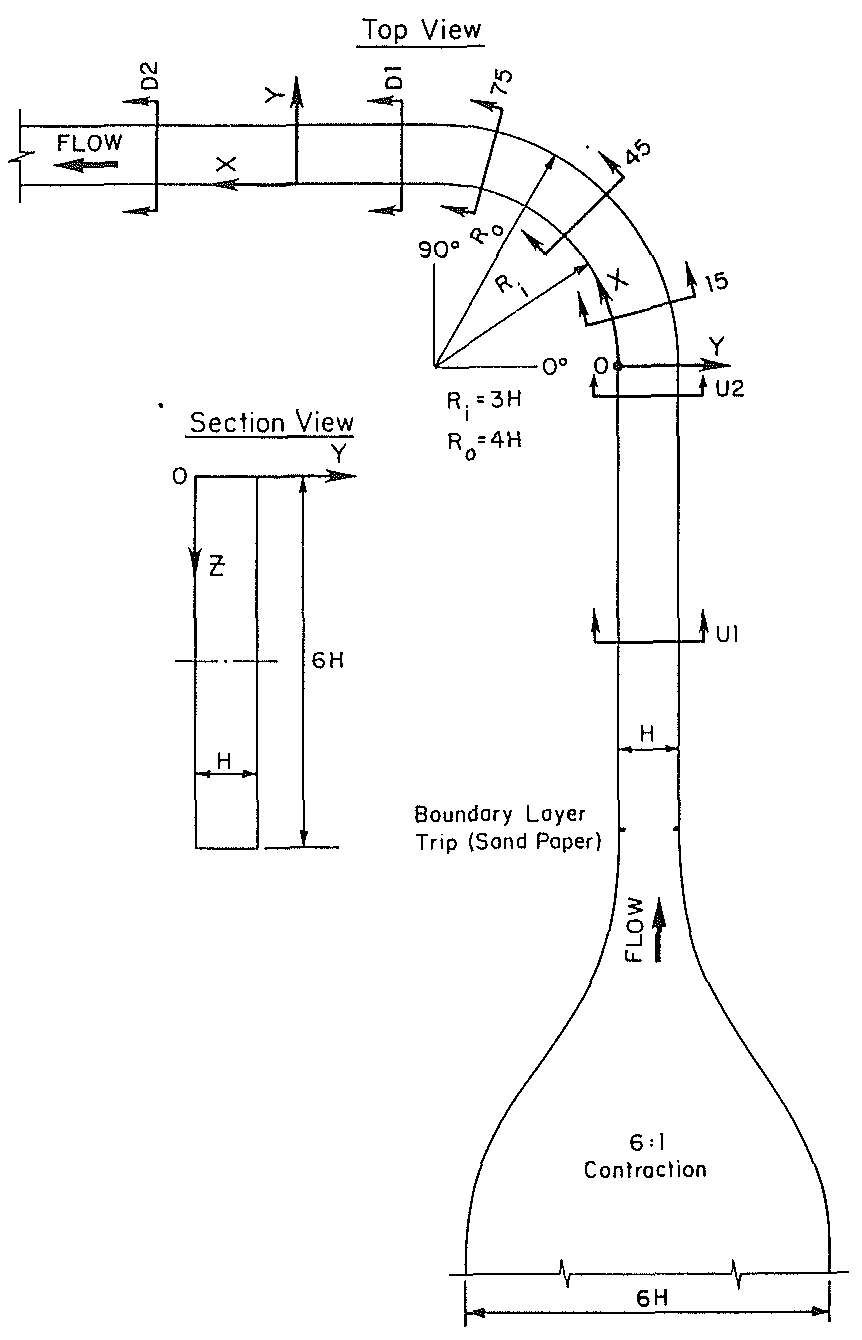
\includegraphics[width=3in]{Kim_Setup.png}
\caption{Experimental geometry of \citet{kim1994}.}
\label{fig:setup_Kim}
\end{wrapfigure}

The main terms involved in $f_{r1}$, shown in \eqref{eq:SARC_definitions}, need to be accessible to the main computation of the eddy-viscosity, also known as the turbulence scalar, source term in \li{e3sourceSclr}. The next changes to the PHASTA source we discuss facilitate this need.

As mentioned in the previous subsection, we require the nodal reconstruction of $S_{ij}$ in order to compute its spatial derivative. The scaled reconstruction, $2 (\nu + \nu_T) S_{ij}$, is called \li{qres}, and its global representation is computed in the flow solve's \li{ElmGMR} routine. We pass the variable up through \li{SolFlow} to \li{itrdrv}, and then down through the increasingly-specific scalar solve routines until we reach \li{e3ivarSclr}. Here, we compute the gradient of \li{qres} (the local version, at least), and divide through by $2(\nu + \nu_T)$ to retrieve the gradient of $S_{ij}$, which is then passed into \li{e3sourceSclr}. The stack of function calls, starting from \li{itrdrv}, is:
\begin{itemize}
\item \li{SolSclr}
\item \li{ElmGMRSclr}
\item \li{AsIGMRSclr}
\item \li{e3Sclr}
\item \li{e3ivarSclr}
\item \li{e3sourceSclr}
\end{itemize}

With this minor change, all additional quantities needed have been passed to \li{e3sourceSclr}. We now consider subsequent terms used in $f_{r1}$. The material derivative of the strain rate tensor can be written as
\begin{equation}
\begin{aligned}
\DD{S_{ij}}{t}
\equiv
\left( \pp{}{t} + u_k \pp{}{x_k} \right) S_{ij}
&=
\pp{}{t}
\left[
\frac{1}{2}
\left( \pp{u_i}{x_j} + \pp{u_j}{x_i} \right)
\right]
+
u_k \pp{S_{ij}}{x_k}
\\
&=
\frac{1}{2}
\left( \pp{}{x_j} \pp{u_i}{t} + \pp{}{x_i} \pp{u_j}{t} \right)
+
u_k \pp{S_{ij}}{x_k}
=
\frac{1}{2}
\left( \pp{a_i}{x_j} + \pp{a_j}{x_i} \right)
+
u_k \pp{S_{ij}}{x_k}
\;,
\end{aligned}
\end{equation}
where the fluid acceleration vector is defined as $a_i \equiv \partial u_i / \partial t$, and we have interchanged the order of derivatives by assuming that $u_i$ varies continuously in space and time. Like $S_{ij}$, $a_i$ is computed during each flow solve. It is already accessible within \li{e3sourceSclr}. We need only calculate two spatial derivative tensors, $a_{i,j}$ and $S_{ij,k}$, contracting the latter with velocity $u_k$, to get $DS_{ij}/Dt$. Such spatial derivatives are computed in the standard manner of \eqref{eq:fem_first_derivs}. We compute $\Omega^2$, $S^2$, and $D^2$ directly in \li{e3sourceSclr} using $u_{i,j}$, which already exists in the code for the standard SA model. Computation of $f_{r1}$ is trivial at this point, and proceeds according to \eqref{eq:SARC_rotation_function}. Changes to the source can be consulted for specific details of implementation.

%%%%%%%%%%%%%%%%%%%%%%%%%%%%%%%%%%%%%%%%%%%%%%%%%
%%%%%%%%%%%%%%%%%%%%%%%%%%%%%%%%%%%%%%%%%%%%%%%%%
\section{Model Validation} %%%%%%%%%%%%%%%%%%%%%%
%%%%%%%%%%%%%%%%%%%%%%%%%%%%%%%%%%%%%%%%%%%%%%%%%
%%%%%%%%%%%%%%%%%%%%%%%%%%%%%%%%%%%%%%%%%%%%%%%%%

Though the changes to PHASTA are relatively straight-forward, they must be validated against existing experimental (and in this case, computational) data. Without validation, application to novel flows would be circumspect.

\subsection{Published Data and Approach}

We validate our implementation against both the experimental data of \citet{kim1994} and the computational data of \citet{shur2000}, both of which concern flow through a 90\degree-bend duct of rectangular cross-section. No system rotation is present.

Kim's experimental geometry is shown in \figref{fig:setup_Kim}. Referencing the top view diagram, flow enters the domain after a contraction section of area ratio 6, and is tripped by sandpaper along all four walls of the duct to generate a fully turbulent boundary layer by the time the flow reaches the bend. The duct has characteristic dimension $H = 8$ in ($0.2032$ m), with inner and outer radii of $R_i=3H$ and $R_o=4H$, respectively. \citet{kim1994} took special care to isolate secondary flows and vortex formation in the corners from purely curvature-driven effects present along the center-line, and accordingly chose a duct aspect ratio of 6. Thus, the span-wise dimension is $H$, and the vertical dimension is $6H$.

\citet{kim1994} report a freestream velocity of $U_0 = 16$ m/s, and a duct Reynolds number of $Re = U_0 H / \nu = 224,000$. This determines the kinematic viscosity to be $\nu = 1.45 \times 10^{-5}$ m$^2$/s. We assume a typical density of air, $\rho = 1.225$ kg/m$^3$.

When presenting our validation data, we use the $X$, $Y$, $Z$ coordinate system of \citet{kim1994}, which locates the origin at the upper inside corner of the duct exactly where it begins to curve. $X$ is the stream-wise coordinate, $Y$ is the span-wise coordinate perpendicular to $X$, and $Z$ is the distance from the top duct wall.

Experimental data is collected at seven measurement stations: U1, U2, 15, 45, 75, D1, and D2, listed in the order they are encountered by a fluid particle in the core of the flow. Stations upstream of the bend are denoted `U', and downstream stations, `D.' In the curved section itself, the angle between the curved-duct centerline and the straight-inflow duct centerline varies from 0\degree to 90\degree. Stations numbered 15, 45, and 75 correspond to those locations. At each station, two measurements are conducted. First, mean streamwise velocity profiles are taken across the $Y$-direction of the duct at $Z/H = \{1,2,3\}$. Second, skin friction values are obtained around half the circumference of the duct cross-section. That is, for a station's fixed $X$-coordinate, $C_f$ is measured at a range of points starting at the center of the inside (convex) wall ($Z/H = 3$), travelling up to $Z/H=0$, across the top wall from $Y/H=0$ to $Y/H=1$, and then back down the outside (concave) wall to the centerline. Combining the $Z/H=3$ measurements also exposes the centerline behavior of $C_f$. These locations can be mapped with a single coordinate $L \in [0,7]$, which denotes the distance around the circumference described above from the starting point. The locations where $C_f$ data may be plotted for maximum informative impact are summarized in \figref{fig:coordinates}.

\begin{figure}[b!]
\centering
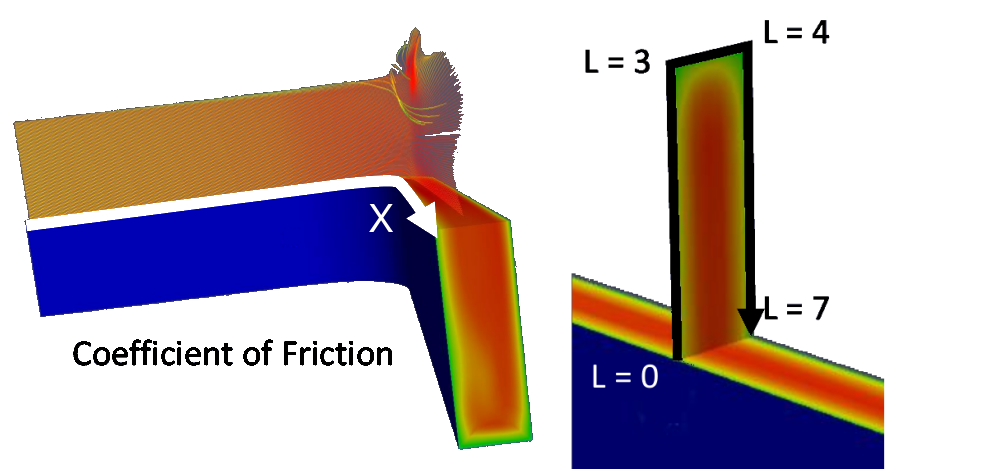
\includegraphics[width=0.6\textwidth]{Coordinate_Systems.png}
\caption{Coordinate systems used for plotting validation data. Left: streamwise coordinate $X$ at duct centerline on inside wall. Right: $L$ describing circumferential distance from inner duct centerline at fixed $X$.}
\label{fig:coordinates}
\end{figure}

In developing the SARC model, \citet{shur2000} validate both their SA and SARC results using this same experiment, and we compare to their results for skin friction coefficient $C_f$. To determine their inlet boundary conditions, the authors ran a straight channel simulation until an adequate turbulent boundary layer developed. These flow and scalar fields were then applied as inflow conditions to their computational domain, which starts at station U1. They used a structured $121 \times 81 \times 61$ grid, resulting in $\sim 600,000$ hexahedral elements. Mesh anisotropy in the straight sections of the duct, which grades to nearly isotropic elements in the curved section, reduces resource requirements of the simulation.

\subsection{Validation Procedure}

\begin{wrapfigure}{r}{3.5in}
\centering
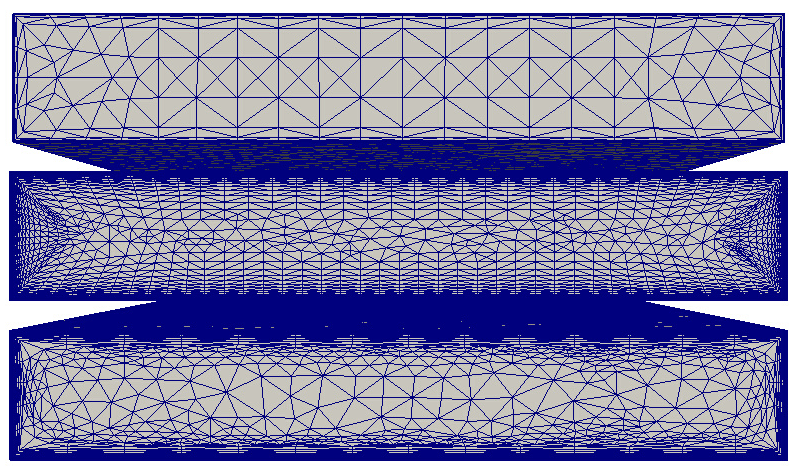
\includegraphics[width=3in]{meshes_bls.png}
\caption{Boundary layer mesh comparison of inflow boundary for meshes A, B, and C (top to bottom).}
\label{fig:mesh_bls}
\end{wrapfigure}

Three main steps comprised our model validation: mesh generation, inflow condition tuning, and analysis of model behavior. There was some interplay between all three. Renderings of the meshes to be discussed are presented in \figref{fig:mesh_overview} and \figref{fig:mesh_bls}. All meshes we create are unstructured.

On all meshes we ran, the boundary conditions applied to the computational domain were, unless otherwise noted:
\begin{itemize}
\item \textbf{Walls:} no slip, zero scalar ($\nu_T$) magnitude
\item \textbf{Outflow:} zero scalar flux
\item \textbf{Inflow:} velocity 13.9 m/s (to grow to the experimental freestream velocity of $U_0 = 16$ m/s at U1's centerline; our inflow velocity was changed to 16 m/s by the end of the process), and a free-stream turbulence value of $\nu_T = 4.35 \times 10^{-5}$, which is $3\times$ the kinematic viscosity, in keeping with \citet{spalart2001}
\end{itemize}

Our first task was to match the experimental velocity profile at station U1. An initial coarse mesh (Mesh~A) was generated for this purpose. It was characterized by an inflow (outflow) straight-section length that far exceeded (matched) the experiment's length of 1.52 m (5.18 m). The upstream section was 7.82 m long to facilitate examination of boundary layer (BL) development. An absolute mesh size of $0.2$ m $\sim H$ was applied, followed by two refinement boxes with absolute mesh sizes of $0.1$ m and $0.05$ m, visible in \figref{fig:mesh_overview}. Boundary layers on all physical walls were added and parametrized by: a first layer height of $\Delta y_1 = 2 \times 10^{-6}$, a total thickness of approximately 1/3 the duct height $\Sigma \Delta y = 0.07$, and 10 total out-of-plane layers. Initial BL development studies determined that the $\Delta y^+_1 \sim 5$ recommendation for coarse or exploratory meshes of \citet{spalart2001} was satisfied, as seen in \figref{fig:initial_yplus}. However, the BL mesh's growth rate was too high to provide adequate out-of-plane resolution for comparison with experimental velocity profile at station U1. This inadequacy of Mesh A is shown in the upper item of \figref{fig:mesh_bls}.

\begin{figure}[b!]
\centering
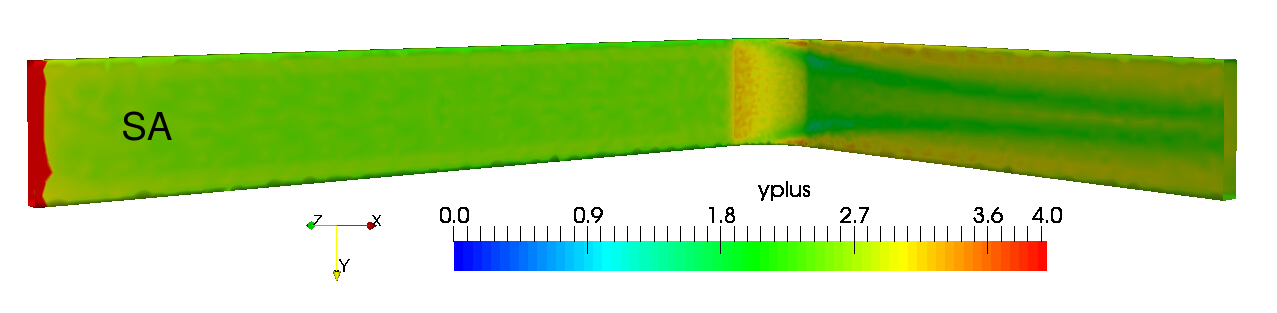
\includegraphics[width=\textwidth]{TuningMesh_Long_yplus.png}
\caption{Un-modified SA model run on Mesh A, with $y^+$ values of the first off-wall mesh points plotted. Maximum value in the curved section is $y^+ \sim 3$. Outer wall has a similar maximum.}
\label{fig:initial_yplus}
\end{figure}

\begin{figure}[p]
\centering
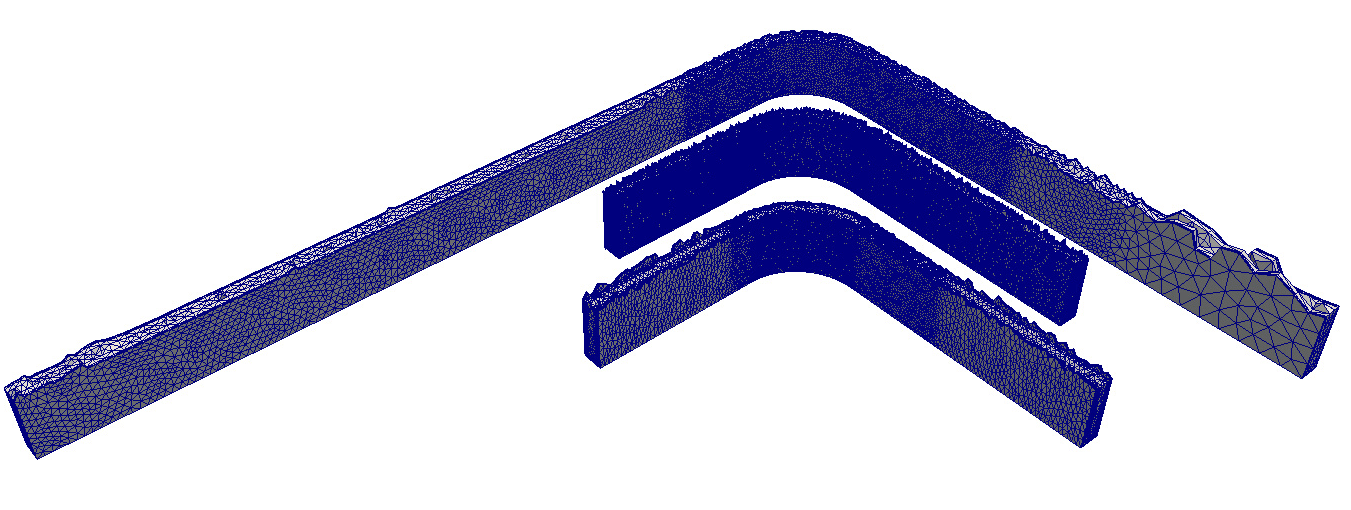
\includegraphics[width=\textwidth]{meshes_far.png}
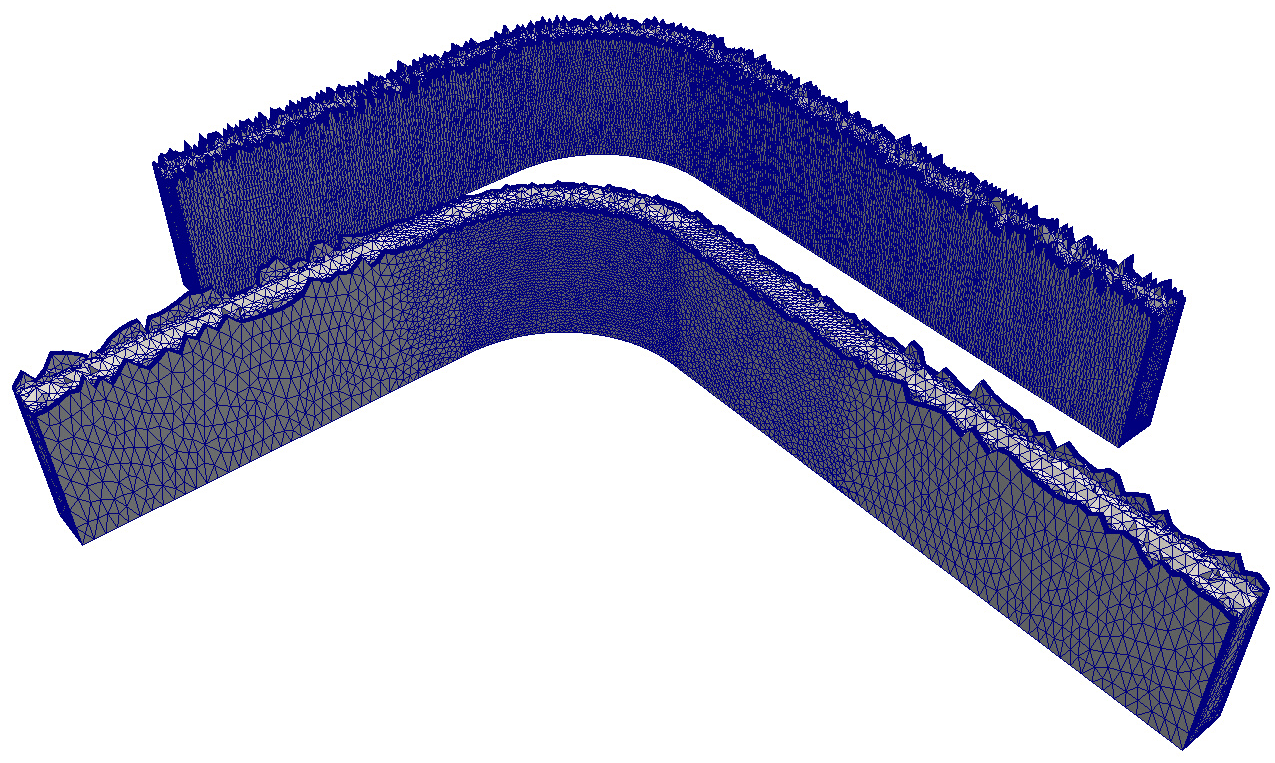
\includegraphics[width=\textwidth]{meshes_zoom.png}\\[1cm]
\caption{Comparison showing the lower half of meshes cut at $Z/H=3$. Upper group of three: meshes A, B, and C (top to bottom). Lower group of two: magnified view of meshes B and C (top to bottom). For all meshes, fluid enters from the left.}
\label{fig:mesh_overview}
\end{figure}

New meshes were made with lower growth rates, primarily by Riccardo Balin. These meshes allowed for detailed comparisons to be made with experimental velocity profiles at U1. Three major conclusions were drawn from this process. First, velocity BL scaling at the inflow had little affect on matching U1 velocity profiles. Second, adding an eddy viscosity profile in the BL helped achieve good agreement with U1 velocities. This scalar profile plays a similar role to the sandpaper trip in the experimental duct, and develops a steeper BL mean velocity gradient. Third and accordingly, the inflow section of the duct could be substantially shortened (see Meshes B and C in \figref{fig:mesh_overview}) because of expedited turbulent BL development. For these later meshes, the value of $\Delta y^+_1$ was iterated upon to meet the recommended value of $\sim 2$ from \citet{spalart2001}. Mesh B and Mesh C, had upstream sections of length 1.69 m, and downstream sections of length 2.5 m. Both had much finer resolution in the $Y$-direction. Mesh B utilized anisotropic elements, but still resulted in 5.25 million tetrahedra, which was too costly for the negligible improvement it showed over our ``final mesh,'' Mesh C. Mesh C was generated with the following properties, and can again be inspected in \figref{fig:mesh_overview}:
\begin{itemize}
\item Anisotropic mesh size of 0.045 m in the $X$- and $Y$- directions, 0.09 m in the $Z$-direction.
\item Refinement box of element edge size 0.03 m
\item Relative curvature refinement with a value of 0.004
\item Boundary layers with $\Delta y_1 = 2 \times 10^{-5}$, $\Sigma \Delta y = 0.027$, and 26 total layers.
\end{itemize}

Runs on Mesh C are conducted with a time step of $1 \times 10^{-2}$ sec, and it takes about 100 time steps to run through the transient. Though transient results may be interesting for debugging purposes, since we are using first-order time integration and such a large time step, they have little physical import.

\subsection{Results and Discussion}

Using Mesh C, we now present results comparing our implementation of the Spalart-Shur curvature correction to those produced by the original SA model.

First and foremost, it is desirable to show evidence that our inflow profile was tuned appropriately to match velocity profiles at U1, and subsequently predict velocity profiles at U2, before effects of curvature come into play. Such profiles are found in \figref{fig:velocity_slices}, and show rather good agreement at all stations and for both models. Exceptions include the outer wall at station 75, where an adverse pressure gradient feeds turbulent mixing and draws high-momentum fluid toward the boundary; and the inside wall at D1, where flow separation occurs due to an adverse pressure gradient at the end of the convex curvature. The adequacy of inflow conditions observed here is consistent with later plots of $C_f$ on the walls of the upstream section.

Eddy viscosity behavior is presented in \figref{fig:ev_slices} and \figref{fig:ev_lines}. Studies on two-dimensional boundary layers indicate that convex curvature has a stabilizing effect on turbulence (i.e. reduces turbulent transport), whereas concave curvature has the opposite effect \citep{kim1994}. Thus, we would expect eddy viscosity to be reduced near the inside wall, while increasing (not necessarily in equal-and-opposite fashion, though) on the outside wall. From \figref{fig:ev_slices} we see this behavior in the SA model results, but not quite for SARC. This is our first warning that the curvature-correction may not be correctly implemented. Though the SARC eddy viscosity increases on the outer wall up until about halfway through the bend, it is rapidly and unexpectedly diminished around station 45. On the inner wall, eddy viscosity appears to stay constant. More quantitative comparison between models in \figref{fig:ev_lines} confirms these trends.

\begin{figure}[h!]
\centering
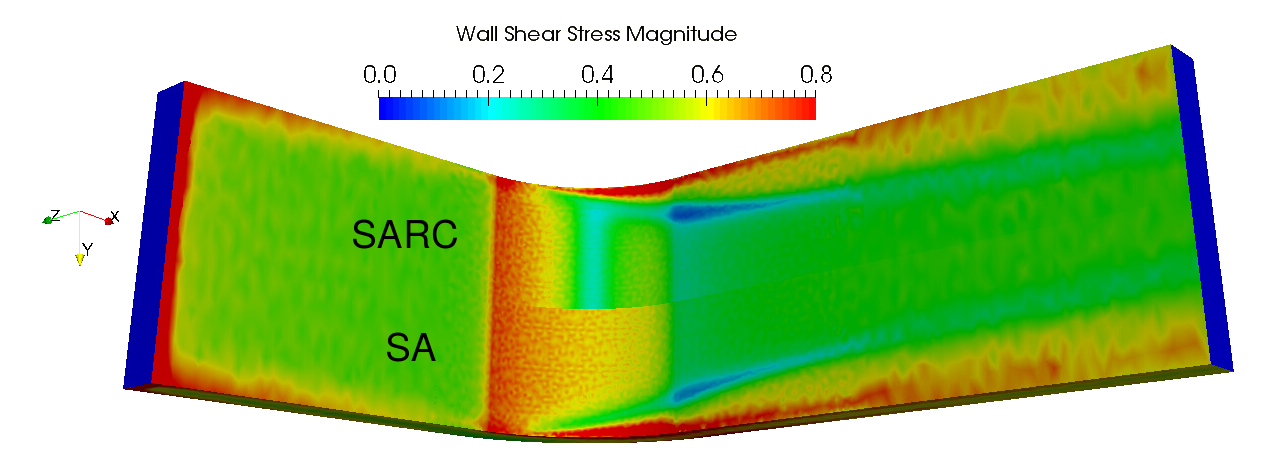
\includegraphics[width=\textwidth]{SA-v-SARC_WallShearStress.png}
\caption{Predicted wall shear stress by SA (bottom) and SARC (top) models.}
\label{fig:wss}
\end{figure}

This odd behavior of the SARC implementation causes strange effects on the wall shear stress shown in \figref{fig:wss}. Though both models show the expected sharp increase in wall shear stress as flow responds to the favorable pressure gradient on the inside wall, the SA model reflects the trend until curvature disappears. Dissimilarly, mid-way through the curved region, SARC predicts a marked drop in wall shear stress, even in the centerline region (not affected by stream-wise corner vortices that develop at the onset of curvature), and despite the fact that the pressure profile remains essentially unchanged for the extent of the curved section.

This does not bode well for our predictions of friction coefficient, since it is just a scaled version of wall shear stress. This is borne out for $C_f$ along the centerline, \figref{fig:Cf_Centerlines}, and along the circumference of each experimental station, \figref{fig:Cf_slices}. The poor performance of both models away from the $Z/H=3$ centerline, corresponding to roughly $2 \le L \le 5$ is expected, since Mesh C simply does not have the requisite corner resolution to capture the secondary flows and vortical structures accurately. On both walls, the SA model seems to do an excellent job of replicating the SA results of \citet{shur2000}.

Though a grid-independence study could be formally conducted, I hesitate to do so for two reasons: first, the implementation is still clearly being debugged, and the current mesh has the ability to capture the ``wrong'' behavior pretty clearly; second, the SA results are nearly identical to those on the 5.25 million-element Mesh B (not shown), and also compare favorably with the results of \citep{shur2000}, which are shown in \figref{fig:Shur_Results}.

\citet{kim1994} also provide pressure coefficient $C_p$ data along the inner and outer walls' centerlines, but we have not used it. Especially for debugging purposes, this could be another useful piece of information.

\section{Conclusion}

In conclusion, it is apparent that our implementation of the curvature-corrected SA model is, unfortunately, still buggy. Before it can be applied to any research cases of interest, these issues will need to be addressed. Nonetheless, the process illustrates some prime difficulties of developing and validating turbulence models. In particular, obtaining a adequate estimate of boundary conditions can be daunting, especially if an experiment does not measure, say, upstream velocity profiles or other relevant parameters. Furthermore, some complex models may not have simple cases on which they can be debugged, and therefore the process of debugging may be extended due resource consumption issues. In any case, I hope to correct the current shortcomings of this SARC implementation in the near future, and hopefully we will produce some interesting results in the near future.

\begin{figure}[p]
\centering
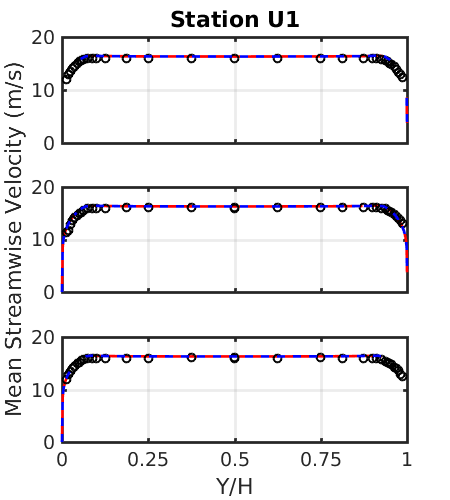
\includegraphics[width=0.32\textwidth]{vel_U1.png}
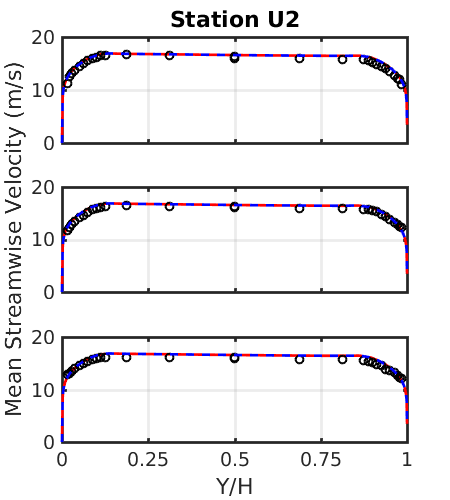
\includegraphics[width=0.32\textwidth]{vel_U2.png}\\
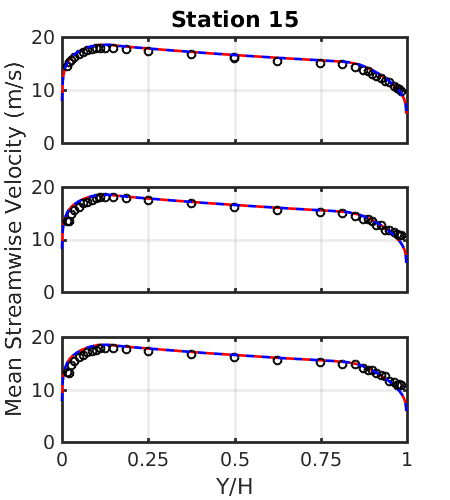
\includegraphics[width=0.32\textwidth]{vel_15.png}
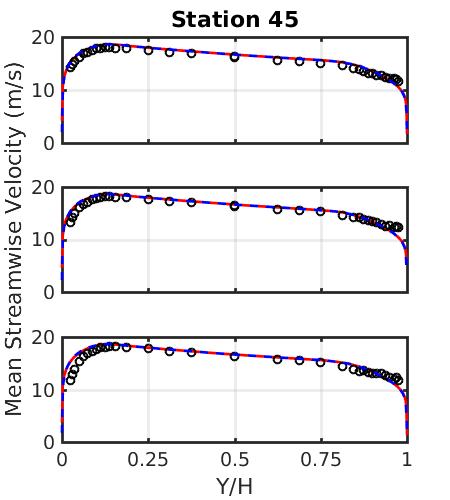
\includegraphics[width=0.32\textwidth]{vel_45.png}
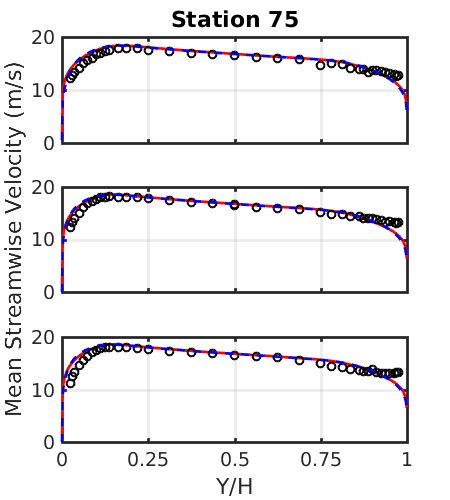
\includegraphics[width=0.32\textwidth]{vel_75.png}\\
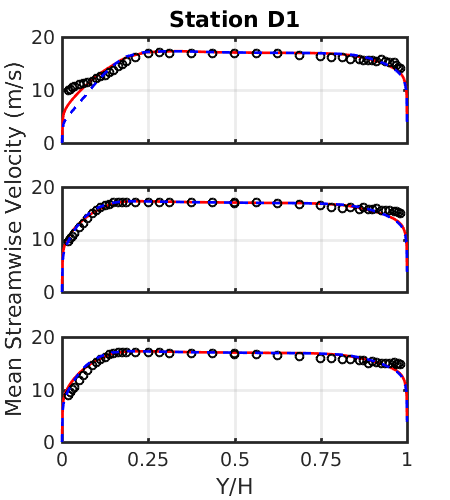
\includegraphics[width=0.32\textwidth]{vel_D1.png}
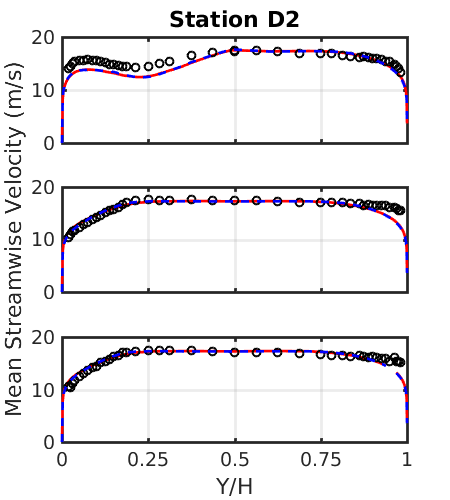
\includegraphics[width=0.32\textwidth]{vel_D2.png}
\caption{Velocity profiles from \citet{kim1994} ($\circ$), and the SA ({\color{blue}\solidrule[6mm]}) and SARC ({\color{red}\dashrule}) models at all seven experimental stations. For each station, velocity profiles are shown at $Z/H = 1, 2, 3$, from top to bottom.}
\label{fig:velocity_slices}
\end{figure}

\begin{figure}[h!]
\centering
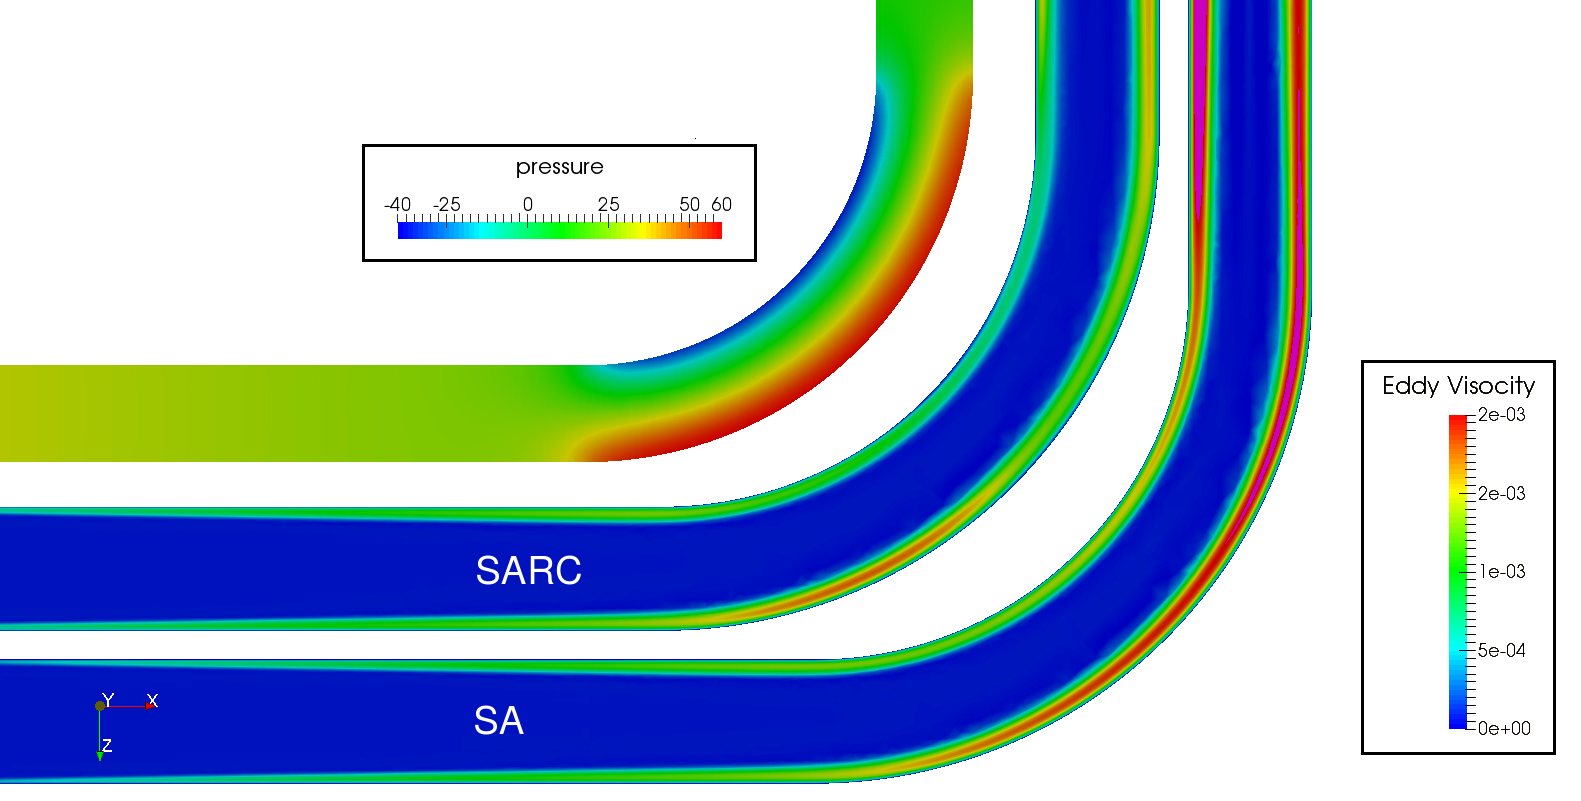
\includegraphics[width=0.9\textwidth]{SA-v-SARC_EddyVisc.png}
\caption{Eddy viscosity (m$^2$/s) behavior comparison between SA and SARC along a centerline slice ($Z/H=3$). Pressure (Pascals) is shown concurrently to understand the de/stabilizing effects of pressure gradient on turbulence in the presence of convex/concave walls.}
\label{fig:ev_slices}
\end{figure}

\begin{figure}[h!]
\centering
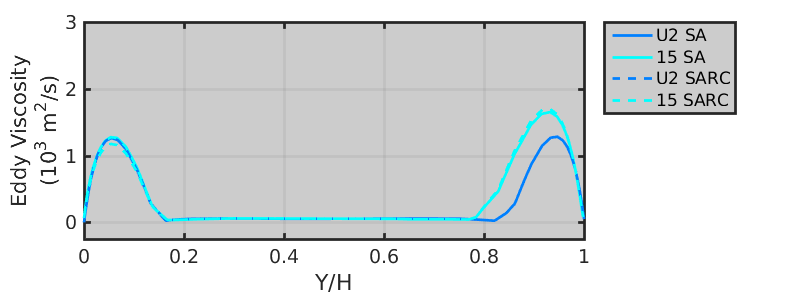
\includegraphics[width=0.75\textwidth]{EV_Comparison_Full_U1_15.png}\\
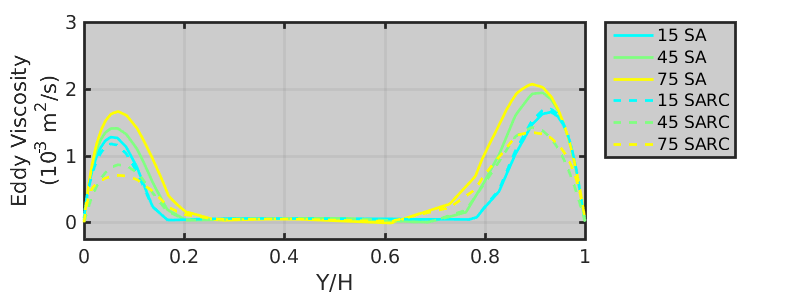
\includegraphics[width=0.75\textwidth]{EV_Comparison_Full_15_45_75.png}\\
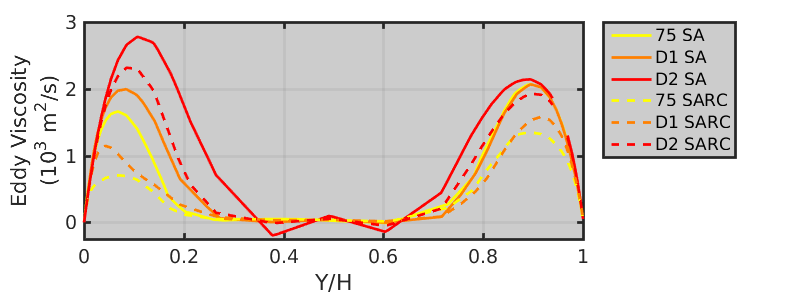
\includegraphics[width=0.75\textwidth]{EV_Comparison_Full_75_D1_D2.png}
\caption{Eddy viscosity behavior comparison between SA (\solidrule[6mm]) and SARC (\dashrule) at $Z/H=3$.}
\label{fig:ev_lines}
\end{figure}

\begin{figure}[h!]
\centering
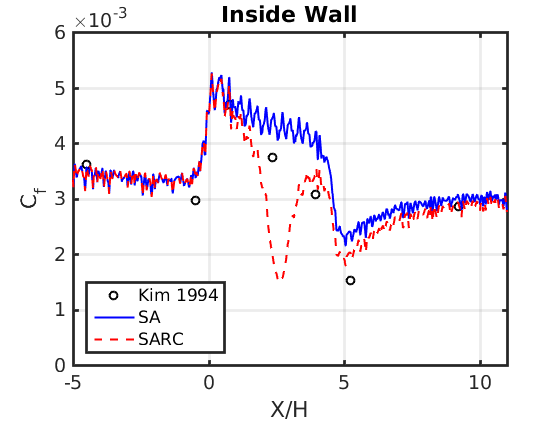
\includegraphics[width=0.48\textwidth]{Cf_Inside_Comparison.png}
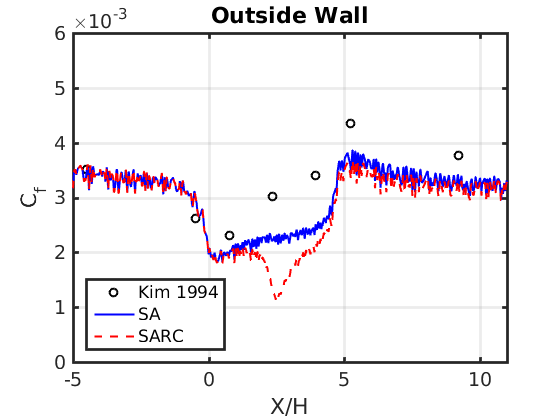
\includegraphics[width=0.48\textwidth]{Cf_Outside_Comparison.png}
\caption{Wall friction coefficient data from \citet{kim1994} ($\circ$), and the SA ({\color{blue}\solidrule[6mm]}) and SARC ({\color{red}\dashrule}) models from $z/H=3$ data at all seven experimental stations.}
\label{fig:Cf_Centerlines}
\end{figure}

\begin{figure}[h!]
\centering
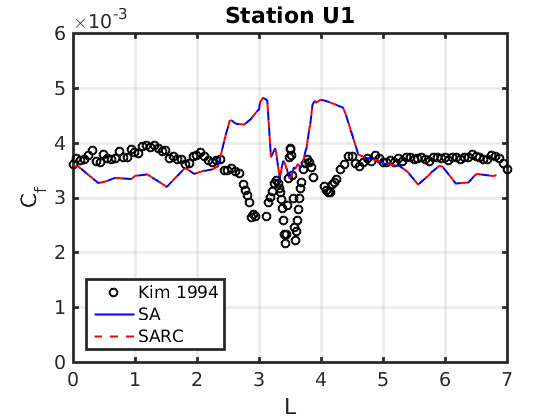
\includegraphics[width=0.32\textwidth]{Cf_U1.png}
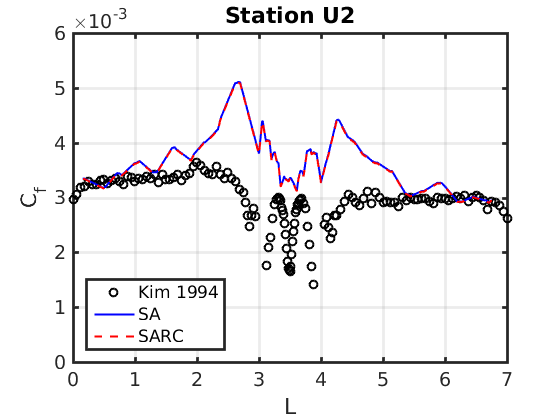
\includegraphics[width=0.32\textwidth]{Cf_U2.png}\\
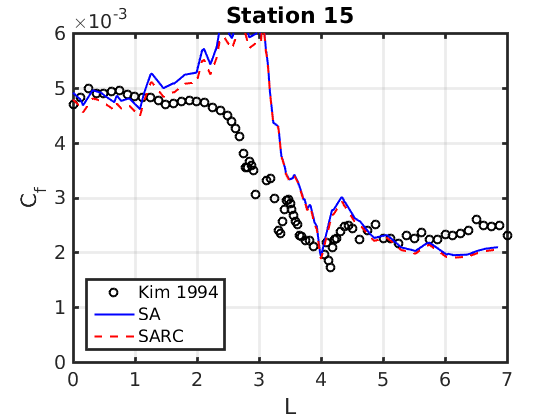
\includegraphics[width=0.32\textwidth]{Cf_15.png}
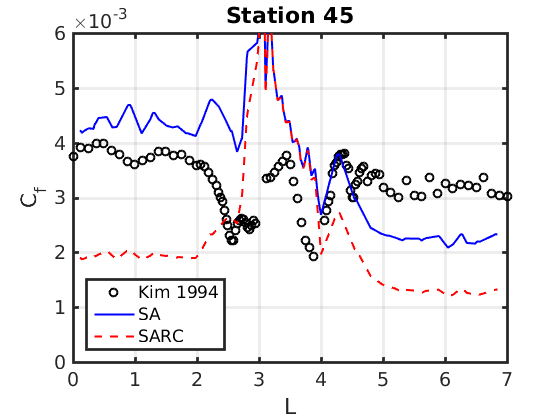
\includegraphics[width=0.32\textwidth]{Cf_45.png}
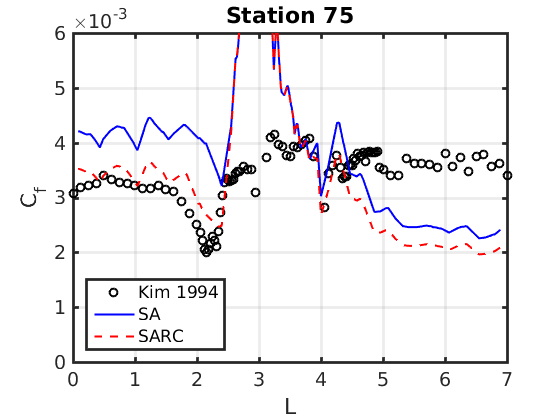
\includegraphics[width=0.32\textwidth]{Cf_75.png}\\
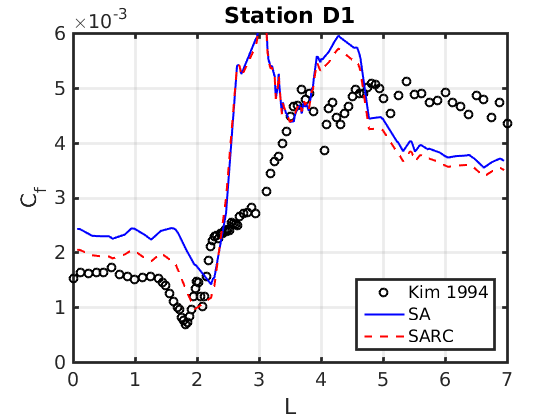
\includegraphics[width=0.32\textwidth]{Cf_D1.png}
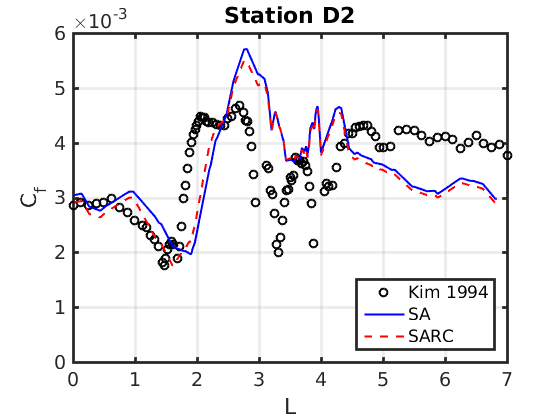
\includegraphics[width=0.32\textwidth]{Cf_D2.png}
\caption{Wall friction coefficient data from \citet{kim1994} ($\circ$), and the SA ({\color{blue}\solidrule[6mm]}) and SARC ({\color{red}\dashrule}) models at all seven experimental stations. $L$ is defined in \figref{fig:coordinates}.}
\label{fig:Cf_slices}
\end{figure}

\begin{figure}[h!]
\centering
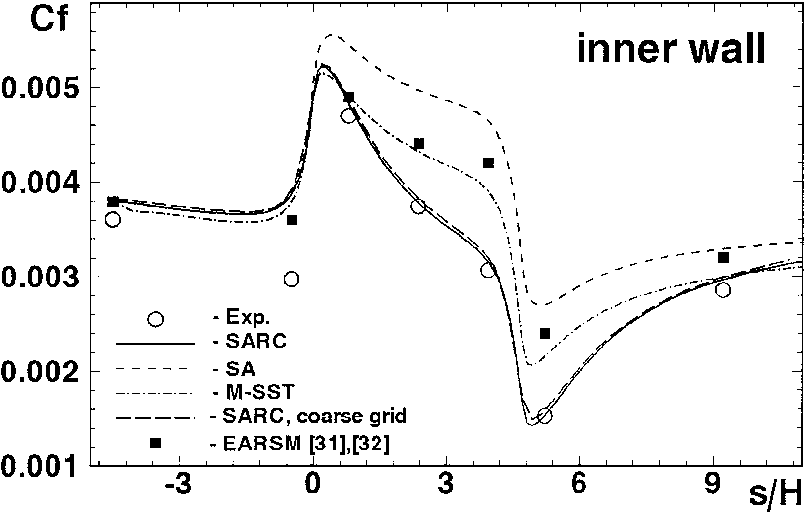
\includegraphics[width=0.48\textwidth]{Shur_FrictionInner.png}
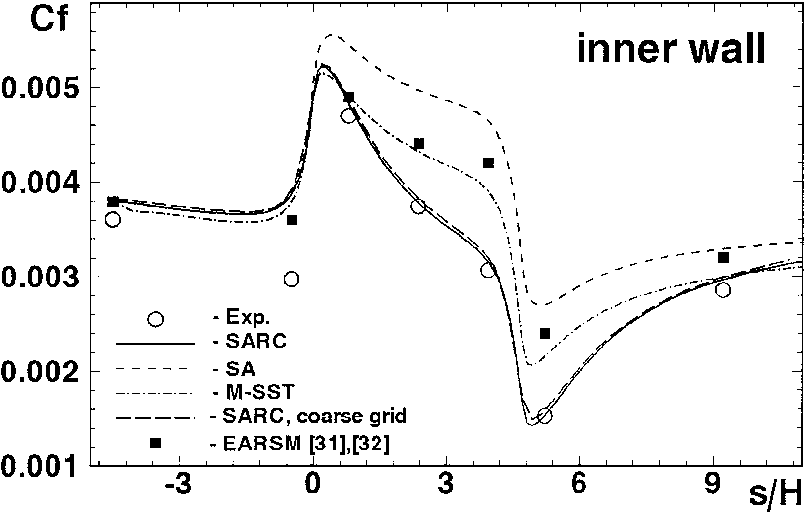
\includegraphics[width=0.48\textwidth]{Shur_FrictionInner.png}
\caption{Centerline friction coefficient results from \citet{shur2000}.}
\label{fig:Shur_Results}
\end{figure}

%%%%%%%%%%%%%%%%%%%%%%%%%%%%%%%%%%%%%%%%%%%%%%%%%
%%%%%%%%%%%%%%%%%%%%%%%%%%%%%%%%%%%%%%%%%%%%%%%%%
%%%%%%%%%%%%%%    BIBLIOGRAPHY    %%%%%%%%%%%%%%%
%%%%%%%%%%%%%%%%%%%%%%%%%%%%%%%%%%%%%%%%%%%%%%%%%
%%%%%%%%%%%%%%%%%%%%%%%%%%%%%%%%%%%%%%%%%%%%%%%%%

\bibliographystyle{plainnat}
\bibliography{sources}

%%
%% DOCUMENT END
%%
\end{document}
